\documentclass[11pt,a4paper,twoside,openright]{report}

% Packages 

\usepackage[english]{babel}
\usepackage[utf8]{inputenc}

\usepackage{amsmath}
\usepackage{amsfonts}
\usepackage{amssymb}
\usepackage{makeidx}
\usepackage{graphicx}
\usepackage{afterpage}
\usepackage{cite}
\usepackage{longtable}

\usepackage[section]{placeins}
\usepackage{float}
\usepackage{listings}
\usepackage{color}

\usepackage{booktabs} % To thicken table lines
\usepackage{pgfplotstable}
\usepackage[final]{pdfpages}


\usepackage[hidelinks]{hyperref}
%\usepackage{minitoc}

\usepackage{cleveref}

\usepackage{geometry} 



\lstset{frame=tb,
	language=R,
	keywordstyle=\color{blue},
	alsoletter={.}
}

\usepackage{enumitem}
\renewcommand\descriptionlabel[1]{\textbf{#1 :}}

\usepackage{subfig}
\usepackage{graphicx}

\usepackage{array}

% Evite les gros début de chapitre inutiles. 
\usepackage{titlesec}

% niveaux de table des matières
\setcounter{secnumdepth}{3}
\setcounter{tocdepth}{3}


\titleformat{\chapter}
{\normalfont\LARGE\bfseries}{\thechapter}{1em}{}
\titlespacing*{\chapter}{0pt}{3.5ex plus 1ex minus .2ex}{2.3ex plus .2ex}

% Modification de commandes 

\newcommand\blankpage{%
	\null
	\thispagestyle{empty}%
	\addtocounter{page}{-1}%
	\newpage}

%\graphicspath{{img}}


\author{Thibault Schowing and Sarah Mcleod}


\usepackage{fancyhdr,graphicx,lastpage}% http://ctan.org/pkg/{fancyhdr,graphicx,lastpage}
\fancypagestyle{plain}{
	\fancyhf{}% Clear header/footer
	\fancyhead[R]{Thibault Schowing and Sarah Mcleod}% Right header
	\fancyhead[L]{Elements of Stastical Learning WS2017/2018}% Left footer
	\fancyfoot[R]{\thepage}% Right footer
}





\begin{document}	
	% Page de titre
	\pagestyle{plain}% Set page style to plain.

	\newgeometry{hmarginratio=1:1}
	
	\pagenumbering{gobble}
	
	\begin{titlepage}
		\centering
		
		%\vspace{0.5cm}
		\small{Saarland University  \par}
		\huge{The Elements of Stastical Learning\par}
		\vspace{1cm}
		
		
		
		\vspace{1cm}
		%MODIFY HERE
		\Large{Assignment 3\par}
		\vspace{1.5cm}
		%MODIFY HERE (day - month - year)
		\small{Due Date: xx.xx.xxxx  \par}
		\vspace{1cm}
		
		
		
		\vspace{2cm}
		\small\textit{Thibault \textsc{Schowing} }Mat. 2571837\par
		\small\textit{Sarah \textsc{Mcleod} }Mat. 2566398\par
		
		\small{\today\par}
		
		\vfill
		
		
	\end{titlepage}
	% Geometry centrée pour page de titre: off
	\restoregeometry 
	%\afterpage{\blankpage}
	
	
	\section*{Problem 1}


\noindent Prove that for linear and polynomial least squares regression, the LOOCV estimate for the test MSE can be calculated using the following formula: 


\begin{equation}
\label{LOOCV_shortcut}
CV_{(n)} = \frac{1}{n} \sum_{i = 1}^{n}\left( \frac{y_i - \hat{y_i}}{1 - h_i} \right)^2
\end{equation}

\noindent Where $ h_i $ is the leverage (3.37, ISLR p98)
\begin{equation}
\label{leverage}
h_i = \frac{1}{n} + \frac{(x_i - \bar{x})^2}{\sum_{i^{'} = 1}^{n} (x_i^{'} - \bar{x})^2}
\end{equation}


\noindent We first have this equation, that can take long if $n$ is big because it has to fit every model.

\[ MSE_i = (y_i - \hat{y_i})^2 \]

\[ CV_{(n)} = \frac{1}{n} \sum_{i = 1}^{n} MSE_i \]


%\noindent The equation \ref{LOOCV_shortcut} is like the ordinary MSE, except the ith residual is divided by $1-h_i$. The leverage lies between $1/n$ and $1$, and reflects the amount that an observation influences its own fit. Hence the residuals for high-leverage points are inflated in this formula by exactly the right amount for this equality to hold.(ISLR, p.180)\\

%$h_{ii}$ correspond to the $i^{th}$ diagonal element of the hat matrix. 

%\[ h_{ii} = [H]_{ii} \]




% https://notesofastatisticswatcher.wordpress.com/2012/12/18/linear-regression-loocv-trick/

\noindent So knowing that $ \hat{y} = Hy $ and as it is a Leave One Out cross validation, we fit $ n $ times the model with one element out. So we have:


\[ H = X(X^T X)^{-1} X^T \]
\[ H^{-i} = X(X^T X)^{-1} X^T_{-i} \]

\noindent The hat matrix with all the data and with one out, respectively

\noindent Then we have
\[ \hat{y}_i = x_i^T [X(X^T X)^{-1} X^T]y \] 
\[ \hat{y}_{-i} = x_i^T [X_{-i}(X_{-i}^T X_{-i})^{-1} X_{-i}^T]y_{-i} \]

\noindent The fitted values at $ x_i$ when using all the data points and when leaving one out. We can then to the following:

\[ \hat{y}_{-i} = \sum_{i\neq j}^{} H_{ij} y_j + H_{ii} \hat{y}_{-i} \]
\[ \hat{y}_{-i} = \sum_{j}^{m} H_{ij} y_j - H_{ii} y_i + H_{ii} \hat{y}_{-i} \]
\[ \hat{y}_{-i} = \hat{y}_{i} - H_{ii} y_{i} + H_{ii} \hat{y}_{-i}  \]


We substitute the in the prediction error: 

\[ y_i - \hat{y}_{-i} = y_i - (\hat{y}_{i} - H_{ii} y_{i} + H_{ii} \hat{y}_{-i} ) \]
\[ y_i - H_{ii}y_{i} - \hat{y}_{-i} - H_{ii}\hat{y}_{-i} = y_i - \hat{y}_i \]
\[ y_i - \hat{y}_{-i} = \frac{y_i - \hat{y}_{i}}{1 - H_{ii}}\]

Taking the mean square error leads to equation \ref{LOOCV_shortcut}. 












	
	\section*{Problem 2}

Show that regression splines of degree d with K knots form a vector space of dimension d + K + 1 by providing a balance of the degrees of freedom in every region of the input data range and the lost degrees of freedom due to the smoothness constraints at the knots. Do not use bases of the spline vector space for your argument.
	
	\section*{Problem 3}
\subsection*{a}


%TODO 



\subsection*{b}
The difference between LDA and QDA is that in QDA, the response variables are still drawn from a Normal distribution but each class has its own covariance matrix. Thus, the posterior probability $ Pr(Y = k | X = x) $ abbreviated $ p_k(x) $ below, cannot be reduced. (4.11 ISLR )

\[ p_k (x) = \frac{\pi_k \frac{1}{\sqrt{2\pi}\sigma_k}exp({-\frac{1}{2\sigma^2_k (x - \mu_k)^2}})}{\sum_{l=1}^{k}\pi_l \frac{1}{\sqrt{2\pi}\sigma}exp({-\frac{1}{2\sigma^2_k (x - \mu_l)^2}})} \]

The denominator here is still constant. It is a sum over all the classes. So, we have to maximize the numerator. We will here consider the log of the numerator and thus we have:

\[ \delta_k (x) = log\left({\pi_k \frac{1}{\sqrt{2\pi}\sigma_k}exp\left({-\frac{1}{2\sigma^2_k (x - \mu_k)^2}}\right)}\right) \]

We expand the $exp()$ content and separate the log and get:

\[ \delta_k (x) = log(\pi_k) - log(\sqrt{2\pi}\sigma_k) - \frac{x^2}{2\sigma^2_k} - \frac{\mu^2_k}{2\sigma^2_k} + \frac{x\mu_k}{2\sigma^2_k} \]

We can see that the $\frac{x^2}{2\sigma^2_k}$ term is quadratic. Because of the $\sigma_k$ values, that are different in opposition with the LDA, it is not possible here to cancel it. So the Bayes classifier here is not linear




	
	\section*{Problem 4}

\begin{enumerate}
	\item From the correlation matrix it looks like displacement, weight, and horsepower all have a high positive correlation with cylinders. Given what we know about cars this makes intuitive sense. Horsepower is most positively correlated with displacement and mpg is most negatively correlated with weight, which, again, makes intuitive sense. 
	\item The scatter plots for three highly correlated variables are below. 
	\newline
	\begin{figure}[htbp]
		\centering
		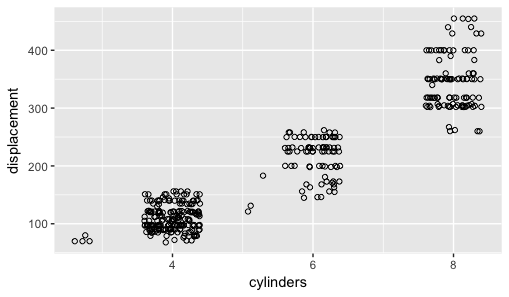
\includegraphics{img/ESL_02_disp_vs_cyl.png}
	\end{figure}
	\begin{figure}[htbp]
		\centering
		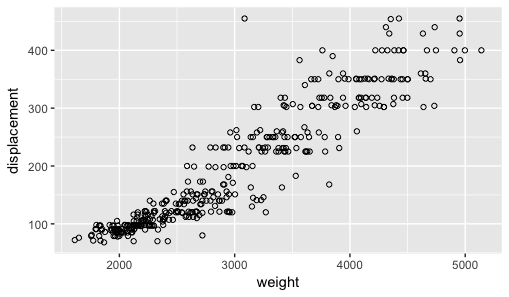
\includegraphics{img/ESL_02_disp_vs_weight.png}
	\end{figure}
	\begin{figure}[htbp]
		\centering
		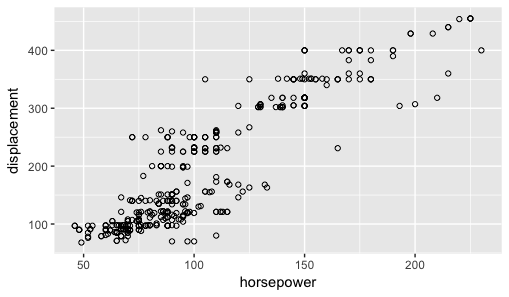
\includegraphics{img/ESL_02_disp_vs_horsepower.png}
	\end{figure}
	\newpage
	Scatterplots for three highly anti-correlated variables are below.
	\begin{figure}[htbp]
		\centering
		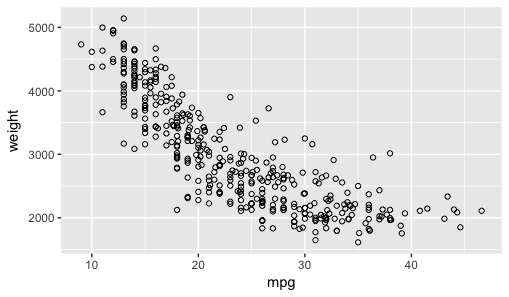
\includegraphics{img/ESL_02_weight_vs_mpg.png}
	\end{figure}
	\begin{figure}[htbp]
		\centering
		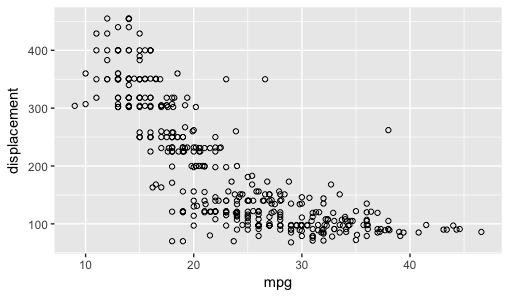
\includegraphics{img/ESL_02_disp_vs_mpg.png}
	\end{figure}
	\begin{figure}[htbp]
		\centering
		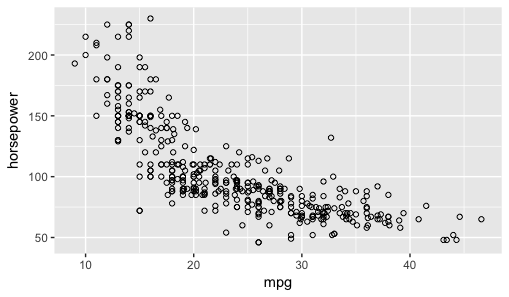
\includegraphics{img/ESL_02_hrsp_mpg.png}
	\end{figure}
	\newpage
	The number of cylinders, the weight of the vehicle, and the horsepower have the highest correlations with displacement, respectively. Some of these numbers make intuitive sense from what we know about how internal combustion engines work. If you want more displacement adding more cylinders is one option to achieve this. Weight, displacement and horsepower are also highly anti-correlated with mpg. So, as the vehicle gets heavier, or gets an increase in power, the efficiency of the engine reduces and you get fewer miles per gallon.
	\newpage
	\item  The p-values show that all of the predictors have a statistically significant relationship to the outcome. From the $R^2$ values displacement as a predictor is a more accurate model. Also, year as a predictor is the least accurate model.  
	\newline
	\begin{tabular}{ccc}
		\centering
		Run Type & $R^2$ & p-value \\
		\hline
		mpg ~ cyl & $0.6047$ & \\
		mpg ~ disp & $0.6482$ &  \\
		mpg ~ hrsp & $0.6059$ &  \\
		mpg ~ year & $0.337$ &
	\end{tabular}
	\item The $R^2$ is 0.8125, which is close to 1. This suggests that this model is an accurate model. Cylinders and horsepower were both statistically significant predictor alone, but in multivariate regression they are not. The coefficients describe the size of the effect of the predictor on the response variable, therefore a negative coefficient gives the amount of decrease in the response for every increase in the predictor.
	\item The residual plot does suggest a non-linearity in the data. The far left side of the plot shows consistent over prediction (i.e. bias) in the data. There don't seem to be any unusually large outliers. There is a high leverage point, point at index 14, as seen in the image below. 
	\begin{figure}[htbp]
		\centering
		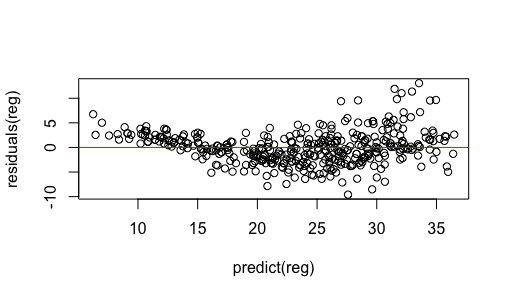
\includegraphics{img/ESL_02_nonlinearity.png}
	\end{figure}
	\begin{figure}[htbp]
		\centering
		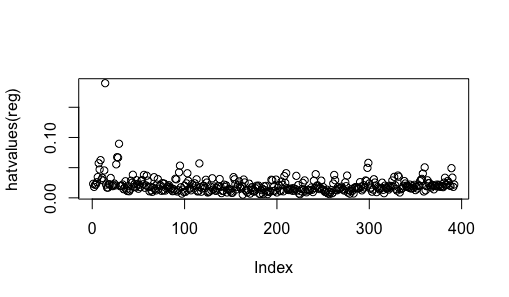
\includegraphics{img/ESL_02_leverage.png}
	\end{figure}
	
	
\end{enumerate}  




	
\end{document}